\chapter{User Documentation}
\label{chap:user-documentation}

This chapter provides user documentation for the CryptoShow application, including a brief introduction on how to use the application.

\section{How to Use}
\label{sec:how-to-use}

To use the CryptoShow application, either deploy it locally (see Section~\ref{sec:deployment}) or access the live version at \url{https://cryptoshow.cz}.

Upon opening the main page, an input table is displayed. Provide either a structure identifier (PDB or AlphaFold ID) or upload a PDB/mmCIF file. Once a valid structure is provided, the application will begin processing and displays the computation status. Processing time varies based on the structure size and server load.

Once the computation is finished, the user is presented with a link to results of the computation. After clicking the link, the user is redirected to the visualization page. The following elements are shown:

\begin{itemize}
    \item An interactive 3D visualization of the structure, allowing users to rotate and zoom. Residues that are part of detected cryptic binding sites are highlighted using distinct colors.
    \item A toolbox providing options to adjust visualization styles.
    \item A table listing the identified cryptic binding sites with expandable rows. Each entry includes details about the involved residues, their scores, and a PyMOL selection string for visualizing the site in PyMOL. For each pocket (in PDB structures), users can initiate an AHoJ query to obtain apo-holo pairs and visualize possible conformational changes. Results can also be downloaded as a ZIP archive.
\end{itemize}

The user interface is shown in Figure~\ref{fig:ui}.

\begin{figure}[htbp]
    \centering
    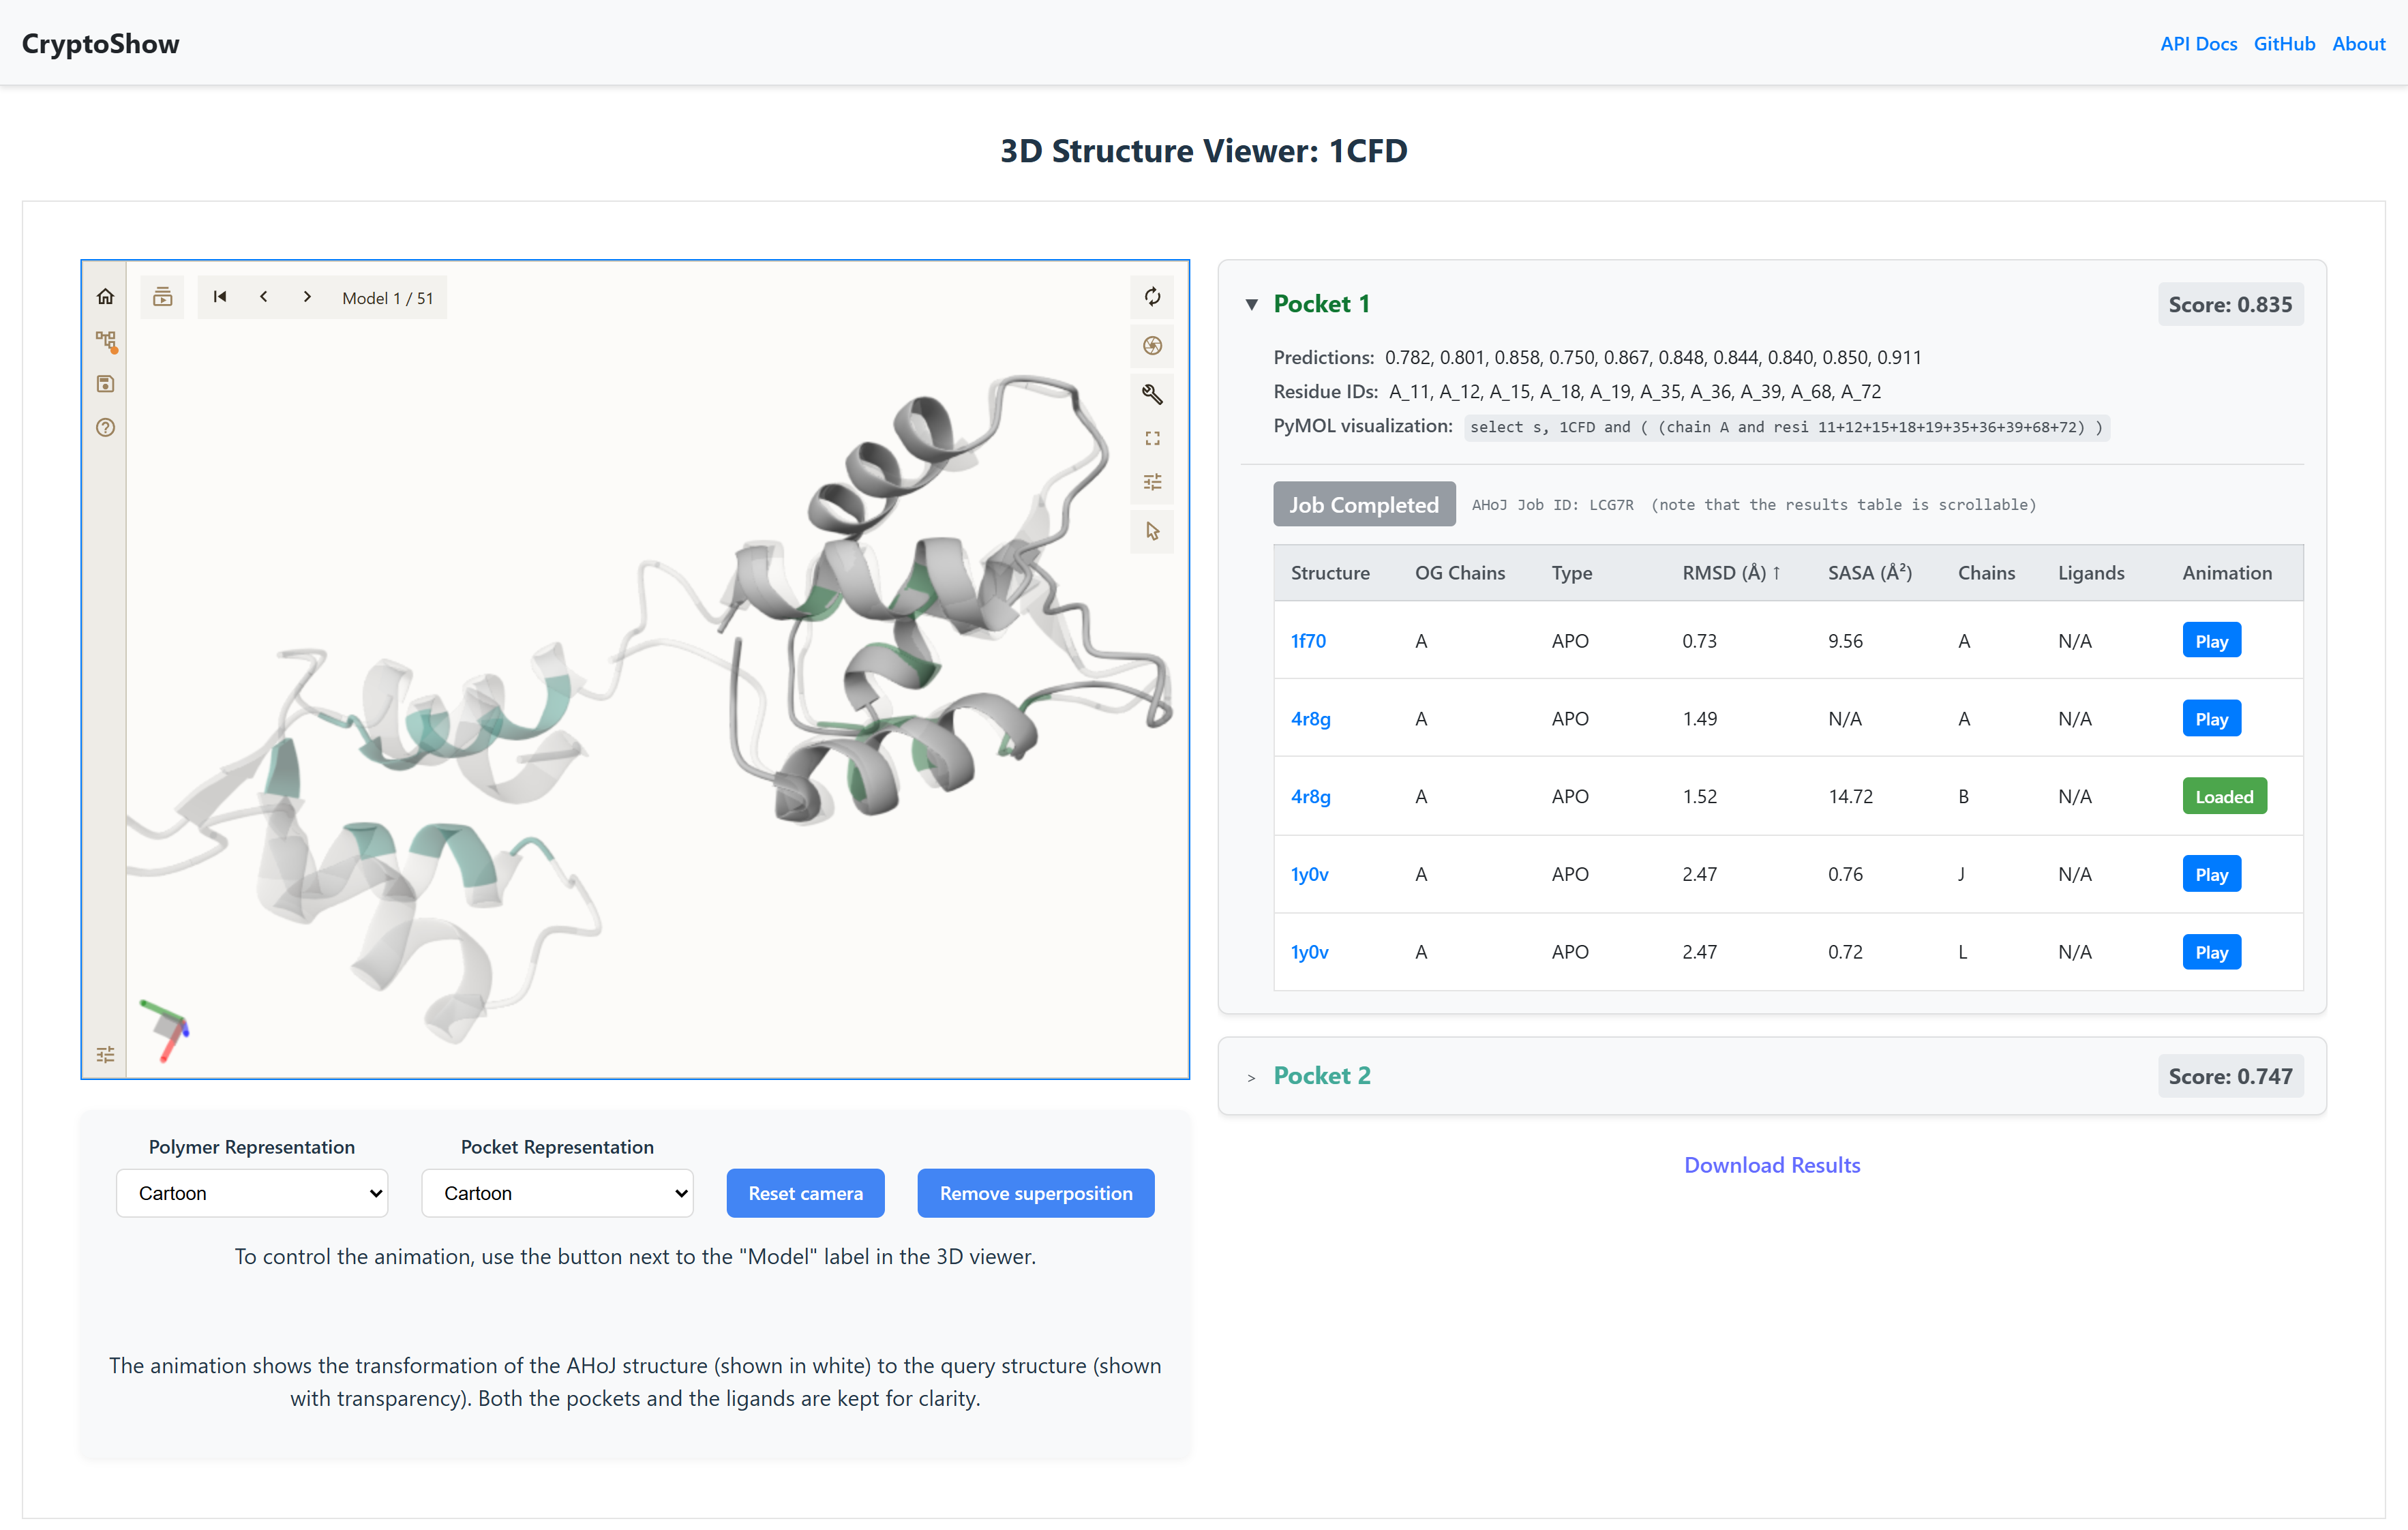
\includegraphics[width=\textwidth]{img/ui.png}
    \caption{User interface of the CryptoShow application. The left side shows the 3D visualization of the protein structure of Calcium-free Calmodulin (1CFD), along with the Crystal Structure of Myosin-1c tail in complex with Calmodulin (4R8G), with the visualization tool box underneath, while the right side displays the table of found cryptic binding sites.}
    \label{fig:ui}
\end{figure}

\section{Use Cases}
\label{sec:use-cases}

\xxx{TODO}
